%!TEX TS-program = xelatex

% Этот шаблон документа разработан в 2014 году
% Данилом Фёдоровых (danil@fedorovykh.ru) 
% для использования в курсе 
% <<Документы и презентации в \LaTeX>>, записанном НИУ ВШЭ
% для Coursera.org: http://coursera.org/course/latex .
% Исходная версия шаблона --- 
% https://www.writelatex.com/coursera/latex/5.2.2

\documentclass[a4paper,12pt]{article}

%%% Работа с русским языком
\usepackage[english,russian]{babel}   %% загружает пакет многоязыковой вёрстки
\usepackage{fontspec}      %% подготавливает загрузку шрифтов Open Type, True Type и др.
\defaultfontfeatures{Ligatures={TeX},Renderer=Basic}  %% свойства шрифтов по умолчанию
\setmainfont[Ligatures={TeX,Historic}]{Times New Roman} %% задаёт основной шрифт документа
\setsansfont{Comic Sans MS}                    %% задаёт шрифт без засечек
\setmonofont{Courier New}
\usepackage{indentfirst}
\frenchspacing

\renewcommand{\epsilon}{\ensuremath{\varepsilon}}
\renewcommand{\phi}{\ensuremath{\varphi}}
\renewcommand{\kappa}{\ensuremath{\varkappa}}
\renewcommand{\le}{\ensuremath{\leqslant}}
\renewcommand{\leq}{\ensuremath{\leqslant}}
\renewcommand{\ge}{\ensuremath{\geqslant}}
\renewcommand{\geq}{\ensuremath{\geqslant}}
\renewcommand{\emptyset}{\varnothing}

%%% Дополнительная работа с математикой
\usepackage{amsmath,amsfonts,amssymb,amsthm,mathtools} % AMS
\usepackage{icomma} % "Умная" запятая: $0,2$ --- число, $0, 2$ --- перечисление

%% Номера формул
%\mathtoolsset{showonlyrefs=true} % Показывать номера только у тех формул, на которые есть \eqref{} в тексте.
%\usepackage{leqno} % Нумерация формул слева

%% Свои команды
\DeclareMathOperator{\sgn}{\mathop{sgn}}

%% Перенос знаков в формулах (по Львовскому)
\newcommand*{\hm}[1]{#1\nobreak\discretionary{}
	{\hbox{$\mathsurround=0pt #1$}}{}}

%%% Работа с картинками
\usepackage{graphicx}  % Для вставки рисунков
\graphicspath{{images/}{images2/}}  % папки с картинками
\setlength\fboxsep{3pt} % Отступ рамки \fbox{} от рисунка
\setlength\fboxrule{1pt} % Толщина линий рамки \fbox{}
\usepackage{wrapfig} % Обтекание рисунков текстом

%%% Работа с таблицами
\usepackage{array,tabularx,tabulary,booktabs} % Дополнительная работа с таблицами
\usepackage{longtable}  % Длинные таблицы
\usepackage{multirow} % Слияние строк в таблице

%%% Теоремы
\theoremstyle{plain} % Это стиль по умолчанию, его можно не переопределять.
\newtheorem{theorem}{Теорема}[section]
\newtheorem{proposition}[theorem]{Утверждение}

\theoremstyle{definition} % "Определение"
\newtheorem{corollary}{Следствие}[theorem]
\newtheorem{problem}{Задача}[section]

\theoremstyle{remark} % "Примечание"
\newtheorem*{nonum}{Решение}

%%% Программирование
\usepackage{etoolbox} % логические операторы


%%% Страница
\usepackage{extsizes} % Возможность сделать 14-й шрифт
\usepackage{geometry} % Простой способ задавать поля
\geometry{top=5mm}
\geometry{bottom=15mm}
\geometry{left=5mm}
\geometry{right=5mm}
%
%\usepackage{fancyhdr} % Колонтитулы
% 	\pagestyle{fancy}
%\renewcommand{\headrulewidth}{0pt}  % Толщина линейки, отчеркивающей верхний колонтитул
% 	\lfoot{Нижний левый}
% 	\rfoot{Нижний правый}
% 	\rhead{Верхний правый}
% 	\chead{Верхний в центре}
% 	\lhead{Верхний левый}
%	\cfoot{Нижний в центре} % По умолчанию здесь номер страницы

\usepackage{setspace} % Интерлиньяж
%\onehalfspacing % Интерлиньяж 1.5
%\doublespacing % Интерлиньяж 2
%\singlespacing % Интерлиньяж 1

\usepackage{lastpage} % Узнать, сколько всего страниц в документе.

\usepackage{soul} % Модификаторы начертания

\usepackage{hyperref}
\usepackage[usenames,dvipsnames,svgnames,table,rgb]{xcolor}
\hypersetup{				% Гиперссылки
	unicode=true,           % русские буквы в раздела PDF
	pdftitle={Заголовок},   % Заголовок
	pdfauthor={Автор},      % Автор
	pdfsubject={Тема},      % Тема
	pdfcreator={Создатель}, % Создатель
	pdfproducer={Производитель}, % Производитель
	pdfkeywords={keyword1} {key2} {key3}, % Ключевые слова
	colorlinks=true,       	% false: ссылки в рамках; true: цветные ссылки
	linkcolor=red,          % внутренние ссылки
	citecolor=black,        % на библиографию
	filecolor=magenta,      % на файлы
	urlcolor=cyan           % на URL
}

\usepackage{csquotes} % Еще инструменты для ссылок

%\usepackage[style=authoryear,maxcitenames=2,backend=biber,sorting=nty]{biblatex}

\usepackage{multicol} % Несколько колонок

\usepackage{tikz} % Работа с графикой
\usepackage{pgfplots}
\usepackage{pgfplotstable}

\author{Батарин Егор}
\title{Алгоритм хэширования Keccak и лавинный эффект.}
\date{}
\begin{document} % конец преамбулы, начало документа
	
	\maketitle
	
	\begin{abstract}
		
		Статья посвящена обзору самому передовому на данный день алгоритму хеширования - Keccak. Рассмотрены история его создания, определение хэш-функции, основные свойства криптографических хэш-функций, общая структура алгоритма Keccak, реализация функции перестановок и описание проекта по исследованию лавинного эффекта на Keccak.
		
	\end{abstract}
	
	\section{История создания алгоритма}
	
	В 2012 году сообщество NIST провело конкурс алгоритмов SHA-3, после того, как были проведены успешные атаки на предыдущие алгоритмы семейства SHA. На конкурс были приняты 51 алгоритмов, в результате естественного отбора которых в качестве нового стандарта SHA был принят алгоритм Keccak.
	
	\section{Что такое хэш-функция?}
	
	Хэш-функция - это отображение, которое ставит в соответствие строке произвольной длины строку фиксированной длины. Как правило, мощность отображаемого множества больше мощности множества значений хэш-функции, а значит она не может быть инъективной. Пара сообщений, нарушающих инъективность функции, называется коллизией.
	
	Сферы применения хэш-функций различны: 
	
	- Построение уникального идентификатора для данного набора данных
	
	- Для вычисления контрольных сумм и обнаружения ошибок
	
	- При сохранении пароля в виде хэш-кода
	
	- При выработке электронной подписи на хэш-код
	
	Последние два применения взяты из криптографии. Не любые хэш-функции годятся для применения в этих случаях. Для этого нужно использовать специальные хэш-функции, называемые криптографическими, которые обеспечивают повышенную безопасность системы.
	
	\section{Свойства криптографических хэщ-функций}
	
	Чтобы хэш-функция была годна для защиты информации, она должна обладать следующими свойствами:
	
	-Сопротивление поиску первого прообраза: для данного хэш-кода трудно найти исходное сообщение, которое было отобращено данной хэш-функцией в данный хэш-код. Иными словами, для данной хэш-функции трудно построить функцию, обратную к ней.
	
	-Сопротивление поиску второго прообраза: для данного сообщения трудно найти другое сообщение, отобращаемое хэш-функцией в тот же хэш-код. 
	
	-Стойкость к коллизиям: нет эффективного полиномиального алгоритма, который находит коллизии.
	
	-Лавинный эффект: малое изменение входных значений хэш-функции сильно меняет выходное значение.
	
	Как правило, криптографические хэш-функции строятся по итеративной последовательной схеме. 
	
	Такая схема позволяет достичь лавинного эффекта, поскольку каждый бит выходного потока зависит от всего входного потока данных. В основе распространенной схемы лежит разделение входного сообщения на множество блоков, каждый из которых обратывается сжимающей функцией. Затем полученное значение используется для последующих итераций. Для того, чтобы длина входного сообщения была кратна длине блока, его удлинняют дополнительными битами до нужной длины. Похожие идеи используются в алгоритме Keccak. Такая констукция называется губкой.
	
	\newpage
	
	\begin{figure}[h!]
		\centering
		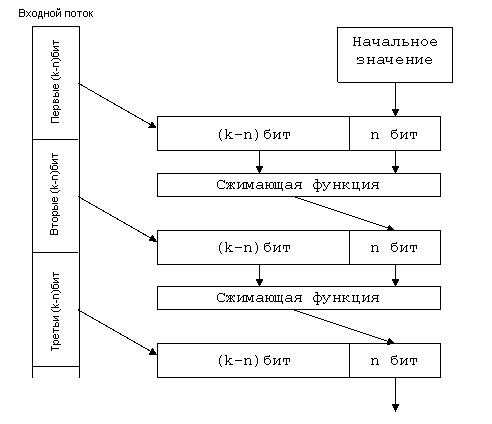
\includegraphics[width=90mm]{1.jpg}
	\end{figure}
	
	\section{Губка} 
	
	Вычисление хэш-кода в констукциях по типу губки происходит в несколько стадий.
	
	\begin{figure}[h!]
		\centering
		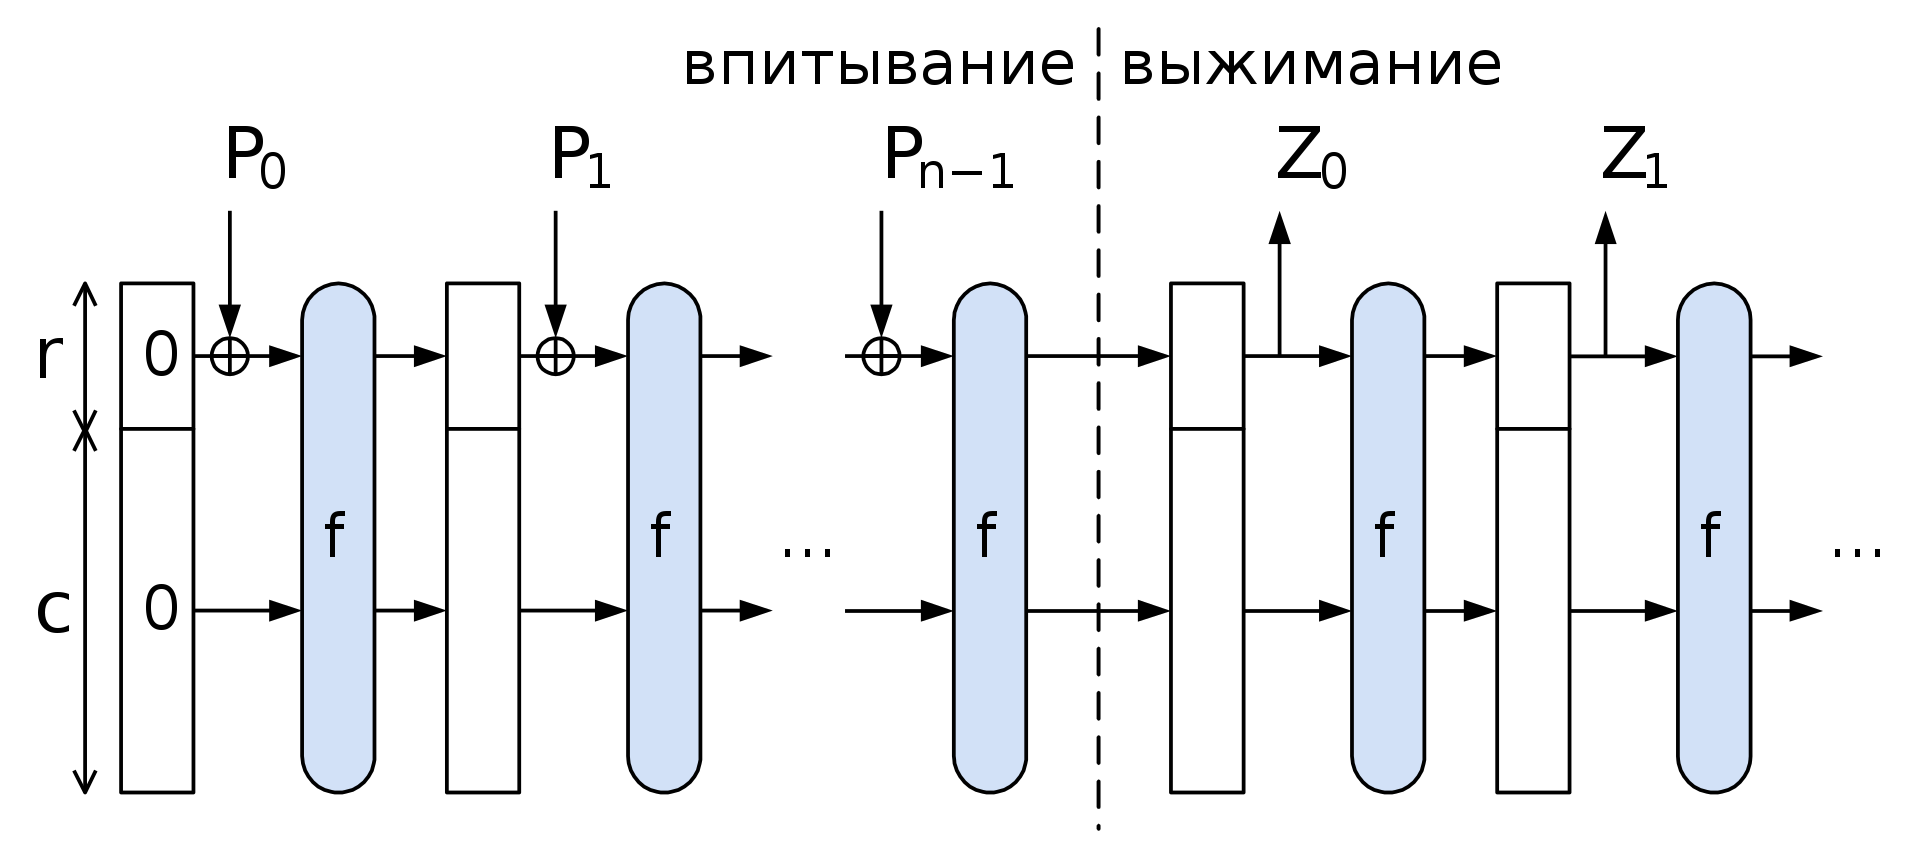
\includegraphics[width=90mm]{2.png}
	\end{figure}

	1) Исходное сообщение $M$ дополняется до строки $P$ так, чтобы длина последнией была кратна $r$. Для этого используется функция дополнения.
	
	2) Строка $P$ делится на строки $P_0$,...,$P_{n-1}$.
	
	3) Происходит этап "впитывания":
	
	3.1) Каждый блок $P_i$ дополняется нулями до строки длины $b$ бит - верхние входы над вертикальными стрелочками на рисунке
	
	3.2) Генерируется начальная строка состояния $S$ длины $b=r+c$, заполненная нулями - самый левый белый прямоугольник на рисунке. 
	
	3.3) Она суммируется по модулю $2$ вместе со строкой $P_0$, а результат обрататывается функцией перестановок $f$.
	
	3.4) Полученная в результате действия $f$ строка длины $b$ суммируется по модулю $2$ с $P_1$ и все последующие операции повторяются итеративно. 
	
	4) Происходит этап "отжимания": на этом этапе суммирование по модулю $2$ прекращается и к строке состояния применяется функция перестановок. К конечному результату $Z$ каждый раз добавляются первые $r$ бит строки состояние. Происходит это ддо того момента, пока длина $Z$ будет не меньше $d$. Когда это достигнуто, лишняя часть обрезается и в конце концов получается строка $Z$ длины $d$.
	
	
	\newpage
	
	\section{Функция перестановок $f$}
	\subsection{Общая структура}
	
	Как мы видели выше, строка состояния $S$ претерпевает изменения под действием функции перестановок $f$ в результате "впитывания" и "отжимания". Авторы представляют эту строку как массив $5 \times 5 \times 64$, стало быть $A[i][j][k]$ - это  $(5i+j)\times 64 + k$ бит строки $S$. В общей реализации SHA-3 вместо $64$ стоит $w = 2^l$, при этом вычисления, проходящие во время определения результата функции перестановок, проходит в несколько раундов, число которых равно $12+2l$ алгоритма Keccak положено $l = 6$, так что для него число раундов равно $24$. В каждый из этих раундов проходит вычисление функций $\theta$, $\rho$, $\pi$, $\chi$, $\iota$. Опишем подробно сущности этих пяти шагов и договоримся на каждом шаге обозначать входной массив за $A$, а выходной за $A'$. $\bmod$ означает сложение по модулю $2$. $i_r$ - номер раунда.
	
	\subsection{Шаг $\theta$}
	
	Для всех $i$ и $k$, таких, что $0 \leqslant i < 5$, $0 \leqslant k < w$, положим
	
	$C(i, k) = A[i, 0, k] \oplus A[i, 1, k] \oplus A[i, 2, k] \oplus A[i, 3, k] \oplus A[i, 4, k]$ 
	
	$D(i, k) = C[(i-1) \bmod 5, k] \oplus C[(i+1) \bmod 5, (k-1) \bmod w]$
	
	Для всех $(i, j, k)$, таких, что $0 \leqslant i < 5$, $0 \leqslant j < 5$, $0 \leqslant k < w$, 
	
	$A'[i, j,k] = A[i, j, k] \oplus D[i, k]$ 
	
	\subsection{Шаг $\rho$}
	
	Для всех $k$, таких, что $0 \leqslant k < w$, $A'[0,0,k] = A[0,0,k]$
	
	Пусть в начале $(i, j) = (1, 0)$. 
	
	Для $t$ от $0$ до $23$ выполнять:
	
	1. Для всех $k$, таких, что 
	$0 \leqslant k < w$, $A'[i,j, k] = A[i, j, (k-(t+1)(t+2)/2) \bmod w]$
	
	2. $(i, j) = (j, (2i + 3j) \bmod 5)$
	
	\subsection{Шаг $\pi$}
	
	Для всех $(i, j, k)$, таких, что $0 \leqslant i < 5$, $0 \leqslant j < 5$, $0 \leqslant k < w$
	
	$A'[i,j,k] = A[(i + 3j) \bmod 5, i, k]$
	
	\subsection{Шаг $\chi$}
	
	Для всех $(i, j, k)$, таких, что $0 \leqslant i < 5$, $0 \leqslant j < 5$,
	
	$A'[i,j,k] = A[i,j,k] \oplus ((A[(i+1) \bmod 5, j, k] \oplus 1) \cdot A[(i+2) \bmod 5, j, k])$
	
	\subsection{Шаг $\iota(A,i_r)$}
	
	Введем дополнительную функцию $rc(t)$. Она вычисляет значения следующим образом:
	
	1. Если $t \bmod 255 = 0$, то возвращается $1$
	
	2. Пусть $R = [1  0  0  0  0  0  0  0]$
	
	3.  Для $i$ от $1$ до $t\mod 255$ выполнять:
	
\qquad	3.1) R = 0 || R
	
\qquad	3.2) $R[0] = R[0] \oplus R[8]$
	
\qquad	3.3) $R[4] = R[4] \oplus R[8]$
	
\qquad	3.4) $R[5] = R[5] \oplus R[8]$
	
\qquad	3.5) $R[6] = R[6] \oplus R[8]$
	
\qquad	3.6) $R = Trunc_8[R]$
	
	4) Возвращается $R[0]$
	
	\newpage
	
	Теперь описываем сам алгоритм $\iota(A,i_r)$:
	
	1. Для всех $(i, j, k)$, таких, что $0 \leqslant i < 5$, $0 \leqslant j < 5$, $0 \leqslant k < w$ $A'[i,j,k] = A[i,j,k]$
	
	2. Положим $RC$ — массив длины $w$, заполненный нулями.
	
	3. Для $i$ от 0 до $l$: $RC[2^i - 1] = rc(i + 7i_r)$
	
	4. Для всех $k$, таких, что $0 \leqslant k < w$, $A'[0,0,k] = A'[0,0,k] \oplus RC[k]$
	
	\subsection{Алгоритм перестановок}
	
	Теперь можно писать структуру всего алогоритма перестановок:
	
	1. Переводим строку $S$ в массив $A$
	
	2. Для $i_r$ от $12 + 2l - n_r$ до $12 + 2l - 1$ применяем $A' = \iota(\chi(\pi(\rho(\theta(A)))), i_r)$
	
	3. Переводим конечный массив $A'$ в строку $S'$
	
	
	\section{Криптоанализ}
	
	На данный момент алгоритм Keccak является самым передомым и надежным среди всех существующих алгоритмов. Тем не менее, существуют известные попытки взлома алгоритма. Рассмотрим некоторые из них.
	
	В работе [7] приводится алгоритм, позволяющий найти коллизии в 384-битной версии алгоритма Keccak с 4 раундами за практическое время $2^{59.65}$. Хотя данный алгоритм неприменим на практике из-за огромного вычислительного времени (иначе пришлось бы разрабатывать SHA-4), он дает существенные продвижения по эффективным аттакам на Keccak, демонстрируя большой выигрыш с предыдущими попытками с практическим временем $2^{147}$. 
	
	Работа [8] представляет алгоритм поиска коллизий уже 6 раундовом алгоритме Keccak c временем $2^{123.5}$, причем с использованием квантовых вычислений достигается ускорение вплоть до $2^{67.35}$.
	
	Аттака на прообраз описана в работе [9]. Здесь аттаки проводятся на алгоритме Keccak 384/512 c использованием линейных структур.
	
	
	
	\section{Применение}
	
	Один из самых ярких примеров использования алгоритма Keccak - криптовалюта Ethereum. Здесь этот алгоритм используется для хэширования Ethereum адресов.
	
	\begin{figure}[h!]
		\centering
		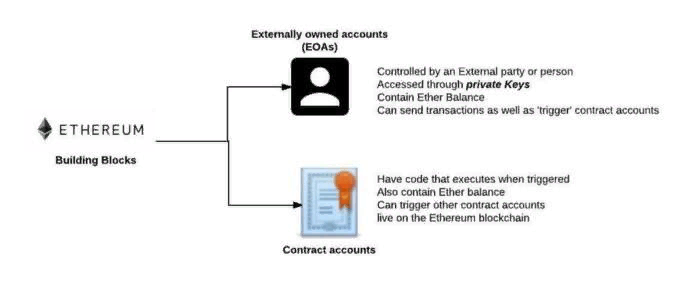
\includegraphics[width=90mm]{3.png}
	\end{figure}
	
	Сами адреса в Ethereum разделяются на два типа:
	
	1) External owned accounts (учетные записи, принадлежащие внешним пользователям, EOA): контролируются закрытыми ключами.
	
	2) Contract accounts (учетные записи смарт-контрактов, CA): самоуправляемы своим своим кодом.
	
	В Ethereum  адрес имеет размер в 20 байт . Он соответствует последним 20 байтам хэша Keccak-256 открытого ключа. Сама процедура создания адреса устроена следующим образом:
	
	1) Создается открытый ключ из закрытого с помощью ECDSA
	
	2) Применяем Keccak к открытому ключу
	
	3) Берем последние 20 байт из хэша - это адрес
	
	\section{Список литературы}
	
	1.\ \href{https://dx.doi.org/10.6028%2Fnist.fips.202}{FIPS PUB 202}

	
	2.\ \href{https://doi.org/10.6028/NIST.SP.800-185}{SHA-3 Derived Functions}
	
	3.\ \href{https://ru.wikipedia.org/wiki/SHA-3}{Статья в Википедии про SHA-3}
	
	4.\ \href{https://habr.com/ru/post/534082/}{Пост в Habr про Keccak}
	
	5.\ \href{https://ru.wikipedia.org/wiki/Хеш-функция}{Статья в Википедии про функцию губки про хэш-функцию}
	
	6.\ \href{https://ru.wikipedia.org/wiki/Функция_губки}{Статья в Википедии про функцию губки}
	
	7.\ \href{https://docs.yandex.ru/docs/view?tm=1670581012&tld=ru&lang=en&name=194.pdf&text=Finding%20Collisions%20against%204-Round%20SHA-3-384%20in%20Practical%20Time&url=https%3A%2F%2Feprint.iacr.org%2F2022%2F194.pdf&lr=213&mime=pdf&l10n=ru&sign=df3555ad7abdca412bd3d1f72d819fd6&keyno=0&serpParams=tm%3D1670581012%26tld%3Dru%26lang%3Den%26name%3D194.pdf%26text%3DFinding%2BCollisions%2Bagainst%2B4-Round%2BSHA-3-384%2Bin%2BPractical%2BTime%26url%3Dhttps%253A%2F%2Feprint.iacr.org%2F2022%2F194.pdf%26lr%3D213%26mime%3Dpdf%26l10n%3Dru%26sign%3Ddf3555ad7abdca412bd3d1f72d819fd6%26keyno%3D0}{Finding Collisions against 4-Round SHA-3-384 in Practical Time}
	
	8.\ \href{https://docs.yandex.ru/docs/view?tm=1670581674&tld=ru&lang=en&name=184.pdf&text=Exploring%20SAT%20for%20Cryptanalysis%3A%20(Quantum)%20Collision%20Attacks%20against%206-Round%20SHA-3&url=https%3A%2F%2Feprint.iacr.org%2F2022%2F184.pdf&lr=214&mime=pdf&l10n=ru&sign=0b0eb5e3f96ac5853b282eebfebc9e20&keyno=0&serpParams=tm%3D1670581674%26tld%3Dru%26lang%3Den%26name%3D184.pdf%26text%3DExploring%2BSAT%2Bfor%2BCryptanalysis%253A%2B%2528Quantum%2529%2BCollision%2BAttacks%2Bagainst%2B6-Round%2BSHA-3%26url%3Dhttps%253A%2F%2Feprint.iacr.org%2F2022%2F184.pdf%26lr%3D214%26mime%3Dpdf%26l10n%3Dru%26sign%3D0b0eb5e3f96ac5853b282eebfebc9e20%26keyno%3D0}{ Exploring SAT for Cryptanalysis: (Quantum) Collision Attacks against 6-Round SHA-3}
	
	9.\
	\href{https://docs.yandex.ru/docs/view?tm=1670582387&tld=ru&lang=en&name=788.pdf&text=Improved%20Preimage%20Attacks%20on%20Round-Reduced%20Keccak-384%2F512%20via%20Restricted%20Linear%20Structures&url=https%3A%2F%2Feprint.iacr.org%2F2022%2F788.pdf&lr=213&mime=pdf&l10n=ru&sign=d880f70fe33c1fb1f84165be0ce9440c&keyno=0&serpParams=tm%3D1670582387%26tld%3Dru%26lang%3Den%26name%3D788.pdf%26text%3DImproved%2BPreimage%2BAttacks%2Bon%2BRound-Reduced%2BKeccak-384%2F512%2Bvia%2BRestricted%2BLinear%2BStructures%26url%3Dhttps%253A%2F%2Feprint.iacr.org%2F2022%2F788.pdf%26lr%3D213%26mime%3Dpdf%26l10n%3Dru%26sign%3Dd880f70fe33c1fb1f84165be0ce9440c%26keyno%3D0}{Improved Preimage Attacks on Round-Reduced
		Keccak-384/512 via Restricted Linear Structures}
	
 10.\ 
 \href{https://habr.com/ru/post/572456/}{Учебник по Solidity. Все об адресах / Хабр}

	

	

	
	
	
	
	
\end{document} % конец документа